\documentclass[11pt,journal,compsoc]{IEEEtran}

\usepackage{ctex}

\usepackage{graphicx}

\usepackage{url}

\usepackage{hyperref}

\usepackage{enumitem}

\usepackage{amssymb}

\usepackage{indentfirst}

\setlength{\parindent}{0em}

\usepackage{float}

\usepackage{minted}

\usemintedstyle{colorful}

\setminted{
    frame=lines,
    breaklines,
    fontsize=\footnotesize
}

\begin{document}


\section{Processors \& Memories}


\subsection{Von Neumann Principle}

程序 和 数据 储存在 单一独立的储存单元 内存 中,它们通过 共同的总线 进行访问。它们在 物理上 是相同的,计算机根据 指令 来处理它们,易重新编程。


\subsection{Von Neumann Loop}

\begin{enumerate}
    \item CPU 从内存中取指令 Fetch
    \item 解码以确定操作 Decode
    \item 执行 Execute
    \item 从内存中取
    \item 写回内存
\end{enumerate}

重复,直到程序结束。CPU 在获取 指令和数据 之间交替,降低速度。


\subsection{Von Neumann Architecture}

存储器、运算器、控制器、输入设备和输出设备五部分组成计算机。运算器和控制器合称为中央处理器。


\subsection{Harvard}

此架构使用 两个不同的储存器 来 分别储存 指令和数据,不同的总线进行访问,速度更快,成本更高。


\subsection{CISC}

Complex / Reduced Instruction Set Computer

复杂指令集的每个指令可执行若干低端操作,指令数目多而复杂,周期长,更适合复杂操作,简单操作可能浪费时间。

原因:寄存器昂贵,尽可能使单个指令做更多的工作


\subsection{RISC}

精简指令集针对流水线化的处理器优化,指令数目少,周期短,更好的并行执行,编译器的效率更高,便宜节能。

x86 对简单指令有硬件加速。

ARM V7 和之前没有 AES。


\subsection{Commands}

一组指示处理器执行特定操作的二进制代码,包含 OpCode 和 Operand 两部分,汇编。


\subsection{Registers}

CPU 内部用来存放临时数据的内存,非常快,很小。x86-64架构有 16 个通用寄存器。

CPU $\leftrightarrow$ 寄存器 $\leftrightarrow$ 缓存 $\leftrightarrow$ 内存


\subsection{Pipeline}

指令流水线,将每条指令分解为多步,每个阶段可以并行执行不同的指令,从而实现几条指令并行处理。指令仍是一条条顺序执行,一个时钟周期内可以执行一条完整的指令。当一个指令在 Execute 时,另一个指令可以开始执行 Decode,以此类推。


\subsection{Superscalar}

在单个核心中有多个流水线,一个时钟周期内执行多个指令,并行地对多条指令进行流水处理。


\subsection{Memories}


\subsubsection{}{按物理结构}

\begin{description}
    \item[SRAM] Field-Effect Transistor、无需刷新、极快、\\ 昂贵、CPU 缓存

    \item[DRAM] Capacitance、周期刷新、内存

    \item[ROM] 只读

    \item[Programmable ROM] 内部有熔丝,利用电流将其烧断,以写入数据,一经烧断便无法恢复

    \item[Erasable PROM] 利用高电压将数据写入,有透明窗口,曝光于紫外线时抹除数据

    \item[OneTime PROM] 与 EPROM 一样,但无透明窗

    \item[Electrically EPROM] 使用高电场来抹除

    \item[Flash] NAND($!\&$ SSD)与 NOR($!\|$ BIOS)型、\\ 寿命有限、较慢
\end{description}


\subsubsection{按组织方式}

\begin{description}
    \item[Serial] 比如 Magnetic Tape、密度高、速度慢、\\ 不能随机存取

    \item[Parallel] 比如 Disk、同时读写多个比特

    \item[Distributed] 信息存储于多个独立且互不干扰的 \\ 设备中、可靠性、扩展性

    \item[Hierarchical] 高效率,比如 Cache -> RAM -> ROM
\end{description}


\subsubsection{按访问类型}

\begin{description}
    \item[Direct Memory Access] 不经过 CPU,比如显卡的 DirectStorage

    \item[Sequential Access Memory] 磁带

    \item[Random Access Memory] 内存
\end{description}


\section{Peripherals \& Storage \& I/O}


\subsection{Storage}

\subsubsection{By Construction}

\begin{description}
    \item[Solid] SSD, Flash 速度快

    \item[Optical] CD, use Laser

    \item[Magnetic] HDD, Tape, Floppy 容量大
\end{description}

\subsubsection{By Operation Principle}

\begin{description}
    \item[RAM] Volatile
    \item[ROM] Non-Volatile
    \item[Sequential]
\end{description}


\subsection{Peripherals}

\subsubsection{By Functionality}

\begin{description}
    \item[Input] Keyboard, Mouse
    
    \item[Output] Monitor, Speaker

    \item[Storage] Flash Drive

    \item[Network] Router, Switch
\end{description}

\subsubsection{By Means}

\begin{description}
    \item[Wired]
    \item[Wireless]
\end{description}

还有 Bidirectional 双向设备


\subsection{Bus}

is physical pathways used by CPU and other devices to communicate.


\subsubsection{Data}

CPU \leftrightarrow RAM

CPU \leftrightarrow I/O Devices

传输数据,宽度决定一次传输多少比特,8 - 64 bits 常见


\subsubsection{Address}

沟通物理地址,宽度决定寻址的内存大小


\subsubsection{Control}

控制 CPU 和设备的:读写、时钟、中断、复位 等信号


\subsection{I/O}

handling is the process of managing the communication between CPU and devices.


\subsubsection{Programmed}

最简单,基本,低效率。CPU 直接控制 I/O 设备和 存储器 之间的数据传输,轮询


\subsubsection{IRQ}

Interrupt-Request。I/O 准备好时,向 CPU 发送中断请求,并处理需求


\subsubsection{Direct Memory Access}


\subsection{Protocols}

传输数据的方法


\subsubsection{Parallel}

所有信号线在同一时刻传输数据 导致信号互相干扰(串扰)。传输速率提高,时钟同步和时序控制变难。

\begin{description}
    \item[Centronics] Enhanced Parallel Port 打印机通信,8 位数据总线和几个控制信号,25 PIN

    \item[Peripheral Component Interconnect] 连接外围设备,32 位 133 MB/s
\end{description}


\subsubsection{Serial}

一次传输一比特,数据沿单一信道传输,差分信号降低干扰和提高质量,增加 Lane 数量提升速率。

差分:一正一负两根线,通过电压差获取数据。

\begin{description}
    \item[Recommended Standard 232] 一条数据线发送接收,控制线用于握手和流量控制,工业

    \item[High-Definition Multimedia Interface] DP

    \item[PCI Express] x32 表示 Lane 数,32 GT/s 每 Lane
\end{description}


\subsubsection{Universal Serial Bus}

同时供电通信,即插即用,40 Gbps,Thunderbolt 兼容

\begin{description}
    \item[主从通信] Host 管理控制数据传输

    \item[层次结构] ~
    
        \begin{itemize}
            \item 物理:接口形状,功率等
            \item 链路:建立和维护通信
            \item 协议:格式等
            \item 传输:打包数据
            \item 会话:管理
            \item 应用:处理驱动程序的请求
        \end{itemize}

    \item[数据包] 传输的基本单位,Token、Data 和 Handshake

    \item[传输模式] ~

        \begin{itemize}
            \item Control:设备配置,状态查询,命令执行

            \item Bulk:大量数据,高速,延迟高

            \item Interrupt:低延迟,少量数据,实时,慢,鼠标

            \item Isochronous:音视频,固定速率和延迟,会丢包
        \end{itemize}

    \item[初始化] 识别设备,查询信息,分配地址,选择配置
\end{description}


\section{Operating Systems}

管理软硬件的软件,为程序提供基本服务,用户与硬件的中介。


\subsection{Classification}

\begin{description}
    \item[Batch] 自动化执行一系列工作(早期大型计算机)

    \item[Time-Sharing] 多用户共享资源,Time-Slicing,为每个用户分配时间片段,并发使用

    \item[Real-Time] 对事件立即作出反应,错过最后期限时:Hard Failure;Soft Tolerable

    \item[Distributed] 超算集群,多合一

    \item[Embedded] 物联网
\end{description}


\subsection{Functionality}

\begin{description}
    \item[管理 Process] 分配 CPU 时间,优先级

    \item[管理 Memory] 虚拟内存,分配内存,内存边界

    \item[File System] 空间分配,控制访问,维护完整性

    \item[管理 Device] 提供标准化接口

    \item[UI] CLI / GUI

    \item[Security] Authentication / Authorization

    \item[Networking] 进程间,网络上

    \item[Error Handling]
\end{description}


\subsection{Process \& Scheduling}

确保资源有效利用,为用户提供灵敏高效的环境


\subsubsection{Process Management}

创建,执行,终止

\begin{description}
    \item[Process] 一个正在执行的程序,由代码、数据和一组资源组成

    \item[Control Block] 包含进程信息,如ID,状态,优先级,内存用量等

    \item[States] 如 ready / running / waiting / terminated

    \item[Scheduler] 根据策略 从就绪队列中 决定哪个进程 应该在指定时间执行
\end{description}


\subsubsection{Scheduling Methods}

\begin{description}
    \item[First-Come, First-Served] 先到先得,对于交互式不佳,可能有长期运行的进程

    \item[Shortest Job Next] 最小化平均等待时间,有可能导致长进程长等待

    \item[Round Robin] 每个进程都有固定的 Quantum 来执行,用完后会被移到队列后方,平衡了公平和效率,适合交互

    \item[Priority Scheduling] 先执行高优先级,确保响应性

    \item[Multilevel Queue Scheduling] 每个优先级都有独立的队列,与其他方法配合

    \item[Multilevel Feedback Queue] 类似上面,但可以根据进程行为,在不同优先级队列中移动进程,比如 I/O 绑定,动态调整提高效率和响应
\end{description}


\subsubsection{Scheduling in Interactive}

优先考虑前台任务,响应性

\begin{description}
    \item[Preemptive Scheduling] 抢占式,可中断运行中的进程,把时间分配给更高优先级,及时响应输入

    \item[Dynamic Priority Adjustment] 根据行为和资源动态调整优先级,如 CPU 爆发式的 I/O 绑定可更优先

    \item[Load Balancing] 在多个 CPU 核心中分配进程,\\ 确保没有过载

    \item[Resource Reservation] 为关键进程保留 CPU 时间

    \item[Adaptive Scheduling] 动态调整使用的策略
\end{description}


\subsubsection{Aim \& Requirements}

\begin{description}
    \item[Fairness] 维持稳定平等,防止垄断

    \item[Efficiency] 最小化开销,最大化吞吐,减少上下文切换,避免 CPU 饥饿

    \item[Responsiveness] 迅速响应高优先级事件

    \item[Predictability] 确保进程在合理的时间内根据优先级和资源需求被执行,实时系统

    \item[Adaptability] 适应不断变化的系统环境,如变化的负载或新进程加入
\end{description}


\subsection{Memory}


\subsubsection{Management}

有效分配,跟踪,管理内存块,使多个进程共享内存并同时执行,确保每个进程有必要的运行资源,防止碎片,进程隔离

\begin{description}
    \item[De / Allocation] 需时分配,用完回收,防止泄漏

    \item[Organization] 将内存分为多个部分,分离不同类型的内存,如 code、data、stack,高效
\end{description}


\subsubsection{Relocation}

调整代码和数据所处的内存地址,允许它在不同的位置执行,多个进程有效分享有限的内存

\begin{description}
    \item[Static] 地址在编译或链接时调整,产物包含最终地址,程序只能在特定地址加载。简单快速但不灵活,一旦加载就不能移动

    \item[Dynamic] 运行时调整地址。加载到内存时会计算实际位置与参考位置的差异,称之为 Relocation Constant 或 Base Address,被添加到程序中每个内存的引用中。允许多个程序共享同一内存空间而不冲突
\end{description}


\subsubsection{Protection}

防止程序非法操作另一个程序的内存,确保稳定性,安全性和完整性。它维持进程隔离,保护敏感数据,防止非法操作导致的系统崩溃。

\begin{description}
    \item[Memory Management Unit] 硬件,将虚拟地址到物理地址。检查进程访问权限,实时内存保护。若有非法访问,则会抛出异常,让操作系统采取行动,如终止进程

    \item[Memory Protection Unit] 硬件,特别是在没有 MMU 或者简单系统中。它定义了具有特定内存访问权限的区域,并检查进程是否有权限

    \item[Virtual Memory] 每个进程都有自己的私有地址空间,与物理层分离,提供额外保护,进程无法直接访问其他内存。OS 管理虚拟内存与物理地址的映射

    \item[Access Control] OS 实现各种访问控制规则,如权限组,以限制进程访问区域

    \item[Address Space Layout Randomization] ~
    
    随机化代码与数据在内存中的位置,使攻击者更难预测布局并执行 Buffer Overflows 等攻击
\end{description}


\subsubsection{Swapping}

Swap 是使用磁盘空间来扩展、释放 RAM 空间的操作,是虚拟内存管理的关键部分。当 RAM 可用不足时,OS 可能会将一些不常用的数据 swapping out 或 paging out,当再次需要时,会被 in 到 RAM。然而这会减慢系统速度,所以 OS 使用复杂的算法,根据频率,内存用量等因素决定哪些部分可以且何时进行交换

\subsubsection{Paging}

将虚拟内存划分为固定大小的块,Pages。物理内存也被划分,Frames。它们具有相同大小,通常是 2 的幂。OS 维护 Page Tables,将 Pages 映射到 Frames,供 MMU 查询。

优点:

\begin{description}
    \item[Efficient Allocation] 通过分块,避免外部碎片,简化操作

    \item[Virtual Memory] 实现的基础

    \item[Protection] 每个进程都有自己的 Page Table,OS 可以为每个 Page 设置权限

    \item[Demand Paging] 只有在实际使用时才加载 Page
\end{description}

开销:

\begin{description}
    \item[Management] Page Tables 需要额外内存和处理

    \item[Translation] 映射开销

    \item[Page Faults] 当引用不在物理内存的 Page 会引发,需要 OS 从磁盘加载,比较缓慢
\end{description}


\section{Network Architectures}


\subsection{Layers}


\subsubsection{Open Systems Interconnection}

\begin{enumerate}
    \item Physical

    电信号,电压,介质规范
    
    \item Data Link

    纠错,流量控制,包含 LLC 和 MAC 两个子层

    \item Network

    不同网络之间的路由和转发,寻址,拥堵控制,数据包排序,IP 在此层

    \item Transport

    可靠端到端传输,错误检查,流量控制,数据分段,TCP 和 UDP

    \item Session

    管理 App 之间的连接,处理中断恢复

    \item Presentation

    处理数据加密,压缩,转换为 App 可理解的格式

    \item Application

    提供接口,高级协议,如 HTTP
\end{enumerate}


\subsubsection{Logical Link Control}

在 一层 和 MAC 层之间提供接口

\begin{description}
    \item[Multiplexing] 增加一个协议标识符,使多个上层协议共享同一个 MAC

    \item[Error Control] MAC 主要处理错误,但 LLC 也可以重传

    \item[Flow Control] 控制速率,防止缓冲区溢出
\end{description}


\subsubsection{Media Access Control}

管理数据如何在介质上传输

\begin{description}
    \item[Addressing] 为设备中每一个接口分配一个唯一的硬件地址,48位,用于识别和引导数据流

    \item[Framing] 将来自上层的内容封装,header(控制,MAC地址)、payload、trailer(校验)

    \item[Error Detection] 使用不同算法检测损坏 Frame,丢弃和重传

    \item[Access Control] 避免冲突,有效利用带宽
\end{description}


\subsubsection{TCP/IP}

TCP/IP 协议是一个协议簇,包含很多协议,UDP TCP ICMP IP...

\begin{enumerate}
    \item Link (1, 2)
    \item Internet (3)
    \item Transport (4)
    \item Application (5, 6, 7)
\end{enumerate}


\subsection{Hardware}

\begin{description}
    \item[Network Interfaces] 1,网卡,通过网络介质传输数据,分配 MAC 地址

    \item[Repeaters] 1,中继,放大信号,扩大覆盖范围

    \item[Bridges] 2,桥接,连接两个独立的网段。根据 MAC 地址,有过滤表,转发数据

    \item[Hubs] 1,集线,连接网络中多个设备,并将数据转发给所有连接的设备,没有过滤等功能

    \item[Switches] 2,交换,连接网络中多个设备,根据 MAC 地址转发和过滤,比 Hub 高效

    \item[Routers] 3,路由,连接多个网络并根据 IP 转发,使用路由算法确定最佳路径,提供 NAT,防火墙,QoS等功能
\end{description}


\subsection{Ethernet}

它是有线 Local Area Network (LAN) 技术,局域网通信标准,1 / 2 层。

\begin{description}
    \item[Topology] 星形结构,设备连接到中央设备,如交换机

    \item[Media] 支持各种介质,Coaxial、Twisted-pair、Fiber-Optic,RJ-45 接口

    \item[Speed] 100 M / 1 G / 10 G 等

    \item[Frame] Preamble, Destination / Source MAC address, EtherType (payload's protocol), Payload (data), Frame Check Sequence.

    \item[MAC] 在传输之前会监听空闲的通道,如果发生多个设备同时传输,则在重试之前会等待一段随机时间
\end{description}


\subsection{802.11 / WiFi}

\begin{description}
    \item[a] 5 GHz,54 Mbps,不易受干扰,范围小

    \item[b] 2.4 GHz,11 Mbps,易干扰,范围广

    \item[g] 2.4 GHz,54 Mbps

    \item[n] 2.4 and 5 GHz,600 Mbps,四个 Spatial 流,MIMO

    \item[ac] 5 GHz,6.93 Gbps,八个流,Multi-User MIMO,同时向多个设备传输,160 MHz 信道,256-QAM

    \item[ax] 2.4 and 5 GHz,9.6 Gbps,OFDMA,BSS Color
\end{description}


\subsubsection{Multiple Input Multiple Output}

发射端的多个天线各自独立发送信号,同时在接收端用多个天线接收并恢复原信息,多根天线增加吞吐量和范围


\subsubsection{Quadrature Amplitude Modulation}

在两个 Orthogonal 载波上进行幅度调制的调制方式,通常是相位差为 90 度的正弦波,星座图上每一个星座点对应发射信号集中的一个信号,星座点数越多,能传输的信息量就越大


\subsubsection{Orthogonal Frequency Division Multiple Access}

将高速的数据流分成多个低速数据流,在多个正交子载波上并行传输


\subsubsection{Basic Service Set Coloring}

标签,用于区分来自不同网络的信号。在高密度环境中,不同 AP 的信号会相互干扰,降低性能。通过为每个 BSS 分配一个颜色标识,减少相邻无线网络之间的干扰


\subsection{Internet Protocol}

不可靠的无连接协议网络协议,不保证交付,不在发送数据前建立连接。第三层,寻址、路由、打包


\subsubsection{IPv4}

Header 最小 20 bytes:

\begin{description}
    \item[Version] 4 bit

    \item[Internet Header Length] 4

    \item[Type of Service] 8

    \item[Total Length] 16

    \item[Identification] 16,Important for Fragmentation and Reassembly

    \item[Flags] 3,—,[1] 保留,[2] 不要分段,[3] 后面还有

    \item[Fragment Offset] 13,—,片段的索引

    \item[Time to Live] 8,在丢弃前最大跳数

    \item[Protocol] 8,TCP 6,UDP 17

    \item[Header Checksum] 16,每一跳都重新计算和校验

    \item[Source IP] 32

    \item[Destination IP] 32

    \item[Options / Padding] var
\end{description}


\subsubsection{IPv6}

IPsec,更好的 QoS,Stateless IP 配置,Multicast and Anycast

定长 Header 40 byte:

\begin{description}
    \item[Version] 4,6

    \item[Traffic Class] 8,QoS

    \item[Flow Label] 20,标记具有相同 QoS 的序列

    \item[Payload Length] 16

    \item[Next Header] 8,如 TCP 头

    \item[Hop Limit] 8,TTL

    \item[Source IP] 128

    \item[Destination IP] 128
\end{description}


\subsection{Network Address Translation}

Types of NAT:

\begin{description}
    \item[Static] 一对一固定公网

    \item[Dynamic] 一对一动态公网

    \item[Port Address Translation] 常用,共享公网
\end{description}

NAT Behavior:

\begin{description}
    \item[Full Cone] 任何外部都可以与映射端口的内部通信

    \item[Restricted Cone] 内部先向外才能通信

    \item[Port Restricted Cone] 相同端口号

    \item[Symmetric] 每一个连接都分配不同的 IP 和 端口
\end{description}


\subsection{Classless Inter-Domain Routing}

无类型域间选路,Classful 是 A (x.0.0.1) B (x.x.0.1) C (x.x.x.1)

子网掩码用于区分网络和主机部分,255.255.255.0 的二进制表示为 11111111.11111111.11111111.00000000,24 个 1 是网络;8 个 0 是主机,则掩码的前缀长度为 24。所以 192.168.1.1 和 255.255.255.0 的 CIDR 为 192.168.1.1/24

127.0.0.0/8 是一个网段,子网掩码为 255.0.0.0。这个网段包含了 127.0.0.0 到 127.255.255.255 的所有 IP 地址。

127.0.0.1/32 是一个单独的 IP 地址,子网掩码为 255.255.255.255,表示只有一个 IP 地址 127.0.0.1。127.0.0.1 也被称为本地回环地址(loopback address)


\subsection{Routing}

路由,在网络中选择路径来发送网络流量的过程,确保数据包能有效和准确地从源头传递到目的地

路由表,存储通往不同网络目的地路径信息的数据结构,当路由器收到数据包时,它在其路由表中查找目的地IP地址,以确定转发数据包的下一跳,它包含:

\begin{description}
    \item[Destination / Mask] 目的地网络,可以是一个地址也可以是网段

    \item[Protocol] 获取到本条路由信息的方式,Direct(0),Static(60),OSPF(10)等

    \item[Preference] 对于不同的 路由协议 进行区分,越低越可靠

    \item[Cost] 某个路由都是从相同的协议收到时,则比较开销,不同协议不可比,越小越优

    \item[Next Hop] 下一个节点

    \item[Interface] 出口设备
\end{description}


\subsubsection{Border Gateway Protocol}

在 Autonomous System 间交换 Network Layer Reachability Information 的协议。当运行于同一 AS 内部时,被称为 Internel BGP,不同 AS 之间时,称为 Externel BGP。

发送 BGP 报文的路由设备称为 Speaker,它接收或产生新的路由,并 Advertise 给其他邻居。BGP 通过 TCP 传递,有Open、Update、Notification (Stop)、Keepalive 和 Route-refresh 五种报文类型


\subsection{Transmission Control Protocol}

Header 20 byte:

\begin{description}
    \item[Source / Des Port] TCP 不记录 IP

    \item[Sequence Num] 解决 Reordering,已传输的字节数会增加它

    \item[Acknowledgement Num] 确认收到

    \item[Flags] 包的类型,操控状态机

    \item[Window] 滑动窗口,流控
\end{description}


\subsubsection{Handshake}

网络上的传输是没有连接的,只有 连接状态。

\begin{description}
    \item[三次握手] SYN - SYN - ACK,同步 Inital Seq Num,用这个序号来拼接数据。

    当服务器在 SYN-RCVD 状态但没有收到最后的 ACK 时,会以翻倍的时间重试。Flood 攻击则是创建大量 SYN 连接并下线,可以把 SYN 队列占满。但可以通过 tcp-syncookies 临时应对:通过 Src Des 和 时间戳 制作一个特殊的 Seq Num 发回去,正常连接会把 SYN Cookie 返回,并直接建立连接

    \item[四次挥手] 其实是两次 FIN - ACK,只不过有一方是被动的。
    
    如果双方同时 FIN,则进入 Closing 状态,等待 Maximum Segment Lifetime (30s) * 2,确保对方收到了 ACK,有足够的时间让此连接不会跟后面的新连接混淆(有些路由会缓存 IP 数据包,如果连接被重用,那么延迟收到的包就可能与新连接混淆)
\end{description}


\subsubsection{重传}

Receiver 发送给 Sender 的 ACK 只能确认最大的连续收到的包,比如发送了 1 2 3 4 5,收到了 1 2,则回复 ACK 3(是期望接收的下一份数据),随后又收到了 4,但是没有收到 3,此时:

\paragraph{Timeout} ~

当 Sender 超时没收到 ACK 3,则

\begin{itemize}
    \item 重传 3
    \item 重传 3 4 5
\end{itemize}

两种方案,但是都要等超时,有可能会很久

\paragraph{Fast Retransmit} ~

所以,不以时间驱动,如果发送方连续收到三次相同的 ACK,就重传

收到 1,回 ACK 2;收到 3,回 ACK 2;4 5 收到,回 ACK 2。则重传 2,回 ACK 6

只解决了时间问题,但是不知道重传一个还是剩下全部

\paragraph{Selective ACK} ~

所以在 TCP 头里面加一个 SACK,汇报已收到的数据,是一个范围。但是 Receiver 有权 Reneging 数据,所以 Sender 也不能完全依赖 SACK,且 SACK 会消耗 Sender 的资源

\paragraph{Duplicate SACK} ~

使用 SACK 告诉 Sender 有哪些数据被重复接收了,让其知道

\begin{enumerate}
    \item 是发出去的包丢了,还是回来的ACK包丢了

    \item Timeout 是否太小了

    \item 网络上出现了 先发的包后到 Reordering 的情况

    \item 网络上是不是把数据包给复制了
\end{enumerate}


\subsubsection{Advertised-Window}

这个字段是 Receiver 告诉 Sender,自己还有多少缓冲区可以接收数据。于是 Sender 就可以根据这个 Receiver 的处理能力来发送数据,而不会导致 Receiver 处理不过来。

如果变成 0 了,则 Sender 会每隔一段时间发送 Zero Window Probe 给 Receiver 来探测对方最新 Window 大小,到一定次数以后会断开连接

Silly Window Syndrome,如果得到的窗口太小了,那么就会当作没有,等到 Window Size >= MSS。如果网络包可以塞满 Maximum Transmission Unit 则可以用满整个带宽,而除去 TCP/IP 头,就得到 Max Segment Size。对于一些需要小包场景的程序,SSH,会关闭 Nagle


\subsubsection{Congestion Handling}

TCP不是一个自私的协议,当拥塞发生的时候,要做自我牺牲

\paragraph{Slow Start} ~

刚加入网络的连接,缓慢地提速

\begin{enumerate}
    \item Congestion Window = 1,表明可以传一个 MSS 大小的数据

    \item 每当收到一个 ACK,cwnd++

    \item 每当过了一个 Round Trip Time,cwnd * 2

    \item Slow Start Threshold 是一个上限,当 cwnd >= ssthresh 时,就会进入 拥塞避免算法
\end{enumerate}

\paragraph{Congestion Avoidance} ~

一般 ssthresh 的值是 65535 kb,当 cwnd 达到这个值时后

\begin{enumerate}
    \item 收到一个ACK时,cwnd + 1 / cwnd

    \item 当每过一个RTT时,cwnd++
\end{enumerate}

\paragraph{当拥塞时} ~

超过 Retransmission TimeOut 则

\begin{itemize}
    \item sshthresh = cwnd / 2
    \item cwnd = 1
    \item 进入慢启动
\end{itemize}


\subsection{User Datagram Protocol}

Header 8 byte:

\begin{description}
    \item[Src Port] 在需要对方回信时

    \item[Des Port] 

    \item[Length] 

    \item[Check Sum] 
\end{description}

特点:

\begin{description}
    \item[无连接] 不维护连接状态

    \item[没有拥塞控制] 可容忍数据丢失,但不能有较大延迟的实时应用

    \item[不可靠] 没有确认 / 重传机制

    \item[面向 Datagram] 应用层来的报文,添加 Header 后直接传递到 IP 层,反之亦然,既不合并也不拆分,不可分割
\end{description}

校验:

UDP 校验和 的计算方法与 IP 的计算方法,都是 二进制反码运算求和 再取反。但不同的是,IP 校验和只检验 IP 数据报 和首部,但 UDP 的校验和是把 伪首部 和 数据 一起校验

有一个伪首部包含

\begin{description}
    \item[Src IP]

    \item[Des IP] 

    \item[0] 

    \item[协议号] 17

    \item[数据报长度] 
\end{description}


\subsection{Quality of Service}

在有限的带宽资源下,QoS 针对网络中有突发流量时需要保障重要业务

业务可以分为:

\begin{description}
    \item[实时] 通常占据固定带宽,对稳定性要求较高

    \item[非实时] 行为难预测,经常出现突发流量,导致网络质量下降,引起拥塞,增加延迟,丢包率
\end{description}

度量指标:带宽,时延,抖动,丢包率


\subsubsection{服务模型}

QoS 模型不是一个具体功能,而是端到端 QoS 设计的一个方案。只有当网络中所有设备都遵循统一的 QoS 服务模型时,才能实现端到端的质量保证。

\begin{description}
    \item[Best-Effort] 最简单模型,用户可以在任何时候,发出任意数量的报文,网络尽力传递,不提供任何保证,适用于要求不高的业务,默认

    \item[IntServ] 在用户发送报文前,需要通过 Signaling 向网络申请特定的 QoS 服务,网络根据请求预留资源。在收到确认信息后,用户才开始发送报文

    其使用了 Resource Reservation Protocol 在整条线路上预留资源,只有所有的网元都确认,路径才能建立

    \item[DiffServ] 将流量分类,享受不同的处理,同一类业务会被聚合起来统一发送,常用

    业务流的分类和汇聚工作在网络边缘节点完成,其通过多种条件,如源 / 目的地址,协议类型等,灵活的对报文进行标记,而其他节点只需要识别报文中的标记,即可进行资源分配和流量控制
\end{description}


\subsection{Domain Name System}


\subsubsection{层级结构}

匿名根 -> 顶级域名 (通用 / 国家)-> 子域

最开始的域名最后都是带了点号的,比如 www.kernel.org. ,表示根域名服务器


\subsubsection{域名服务器}

\begin{description}
    \item[根] 全球共有 13 个不同 IP 地址的最高层次的域名服务器,从 a 一直到 m,ICANN,Anycast

    根 NS 知道所有的 顶级 NS 的地址。向 Root 请求解析 aloen.to,则会返回 .to 的 Top NS,再向其请求 aloen 的 DNS 记录

    \item[顶级] 负责该顶级域名下注册的二级域名解析

    \item[Authoritative] 子域名解析

    \item[本地] 主机发出 DNS 查询时,首先发给本地 NS
\end{description}

查询 DNS 但服务器没有结果:

\begin{description}
    \item[Iterative] DNS 服务器询问其他服务器
    \item[Recursive] 返回另一个 DNS 服务器地址
\end{description}


\subsubsection{常见记录类型}

\begin{description}
    \item[Address] 映射到 IPv4

    \item[AAAA] IPv6

    \item[Canonical NAME] 映射到另一个域名,别名

    \item[Mail Exchange] 射到邮件服务器

    \item[NS] 指定该域名的授权域名服务器

    \item[TXT] 存储关于域名的任意文本信息

    \item[Pointer] IP 反查
\end{description}


\section{Network \& Security}


\subsection{Data Security}

数据 Integrity,Confidentiality 和 Availability

\begin{description}
    \item[Encryption]
    \item[Access Control]
    \item[Backup]
    \item[Data Loss Prevention Tool] 检测和防止敏感数据的非法转移和泄露
    \item[Data Masking] 使用虚构的数据替换敏感信息
\end{description}


\subsection{Service Security}

免受如 APP,API 的未经授权访问或破坏与漏洞

\begin{enumerate}
    \item 定期进行漏洞扫描和补丁

    \item 在软件开发时进行安全测试

    \item 部署防火墙,IDS,IPS

    \item 网段隔离

    \item 对设备和程序进行安全配置
\end{enumerate}


\subsection{Physical Security}

防止盗窃,损坏,未经授权的访问

\begin{description}
    \item[安全设施] 访问控制,监控摄像,报警器

    \item[访问控制系统] 读卡器,生物识别等

    \item[安保人员] 监视和 Patrol

    \item[环境控制] Fire Suppression Systems,Uninterruptible Power Supplies,Air Conditioning

    \item[Asset Management \& Tracking]
\end{description}


\subsection{Security Risks of the Internet}

\begin{description}
    \item[Data Breaches] 未经授权的访问,导致身份信息被盗,财产损失等

    \item[Malware] Viruses, Worms, Trojans, Ransomware, Spyware

    \item[Social Engineering]

    \item[Distributed Denial of Service] 流量攻击

    \item[Insider Threats] 员工权限滥用
\end{description}


\subsection{Classic Encryptions}

\begin{description}
    \item[Caesar Cipher] 偏移替换,每个字母都有固定替换

    \item[Vigenère] 由一些偏移量不同的凯撒密码组成
\end{description}


\subsection{Symmetric Cryptography}


\subsubsection{Advanced Encryption Standard}

密钥长度可以是 128 192 256 位,加密过程简单描述:

\begin{description}
    \item[SubBytes] 将明文中每个字节替换成一个固定的,从 S盒 中查到的值
    
    \item[ShiftRows] 将每行的字节循环位移,使得每个字节都出现在不同的列

    \item[MixColumns] 将每列中的字节进行线性变换,使得每个字节都参与到混淆中

    \item[AddRoundKey] 将每一轮的密钥与每个字节进行异或操作,以增加强度
\end{description}

128 位的密钥 10 轮加密,192 位 12 轮,256 位 14 轮

在逆变换中,只有 AddRoundKey 与加密过程相同


\subsubsection{Substitution Box}

代换盒,由一张固定的表格构成,用于将输入的位序列映射到输出的位序列。在 AES 中,S 盒是通过多种加密学原理和技术精心构造的,以确保其具有良好的加密性质和统计性质。其包含了 256 个元素,每个元素都是一个 8 位的二进制数


\subsection{RSA}

三个人名

组成:

\begin{description}
    \item[Message] $M$

    \item[Ciphertext] 密文 $C$

    \item[Public / Private] Key

    \item[Encryption / Decryption] 算法
\end{description}

产生密钥:

\begin{enumerate}
    \item 随机选择两个不同的素数,$p = 103$,$q = 97$

    \item $n = p * q = 9991$

    \item 计算欧拉函数 $\varphi(n) = (p - 1)(q - 1) = 9792$

    \item 随机选择一个 $e = 1213$,$\varphi(n)$ 与 $e$ coprime ($gcd(a, b) = 1$) 且 $1 < e < \varphi(n)$

    \item 求 $ed - k\varphi(n) = 1$ 整数解:$k = 510, d = 4117$

    \item 公钥 (e, n) = (1213, 9991)
    
    \item 私钥 (d, n) = (4117, 9991)
\end{enumerate}

加密:

令 $M = 6$,得到 $C = M^e (mod ~n)$

$= 6^{1213} (mod ~9991) = 7863$

解密:

$M = C^d ~mod ~n = 7683^{4117} ~mod ~9991 = 6$


\subsection{Diffie-Hellman}

基于 Discrete logarithm Problem 的困难性

\begin{enumerate}
    \item 双方协商 大质数 G 和 Primitive Root N

    G = 13,N = 7

    \item 甲 选择一个私有整数 a = 2

    $A = G^a ~mod ~N = 13^2 ~mod ~7 = 1$

    \item 乙 选择一个私有整数 b = 3

    $B = 13^3 ~mod ~7 = 6$

    \item 双方交换 A B

    \item 甲 使用 B 计算密钥

    $K = B^a ~mod ~N = 6^2 ~mod ~7 = 1$

    \item 乙 使用 A 计算密钥

    $K = A^b ~mod ~N = 1^3 ~mod ~7 = 1$
\end{enumerate}


\subsection{Social Engineering}

\begin{description}
    \item[Phishing] Fraudulent Emails or Messages

    \item[Baiting] 虚假中奖信息

    \item[Tailgating] 尾随进入门禁

    \item[Impersonation] 冒名顶替

    \item[Dumpster Diving] 翻找目标的垃圾以获取信息

    \item[Shoulder Surfing] 在对方输入敏感信息时,从旁边观察

    \item[Reverse] 让目标相信他们需要帮助
\end{description}


\subsection{Brute-Force Attack}

\begin{description}
    \item[Dictionary] 常见组合

    \item[Hash Collision] 生成与原始内容具有相同哈希值的数据,加 Salt

    \item[Rainbow Table] 预先计算好的哈希表来查找明文密码
\end{description}


\subsection{Analytical Attack}

\begin{description}
    \item[Differential Cryptanalysis] 分析多个值的差异,寻找算法模式

    \item[Implementation] 寻找软件或硬件漏洞,Buffer Overflow

    \item[Side-Channel]
\end{description}


\subsection{Firewall}

基于一组安全规则来监视和控制网络流量,FW 决定是否允许流量通过,可以内置于硬件,软件,或者组合,来保护安全。不受信任的网络是互联网。FW 也可以用于内容过滤,例如学校可以配置防火墙以防止有害内容。


\begin{description}
    \item[Packet-filtering] 网络层,根据规则过滤检查包头,速度快,不能提供复杂攻击保护

    \item[Stateful] 网络层,跟踪活动连接状态,通过上下文,提供比包过滤更精细的控制
    
    \item[Proxy-based] 应用层,充当代理,当许多人同时访问时,性能会下降,导致延迟

    \item[Next] 除以上功能外,使用 DPI 在更深层次上检测数据,识别和阻止隐藏在看似正常的流量中的威胁
\end{description}


\subsubsection{Intrusion Detection Systems}

依照一定的安全策略,对网络、系统的运行状况进行监视,尽可能发现各种攻击企图、攻击行为或者攻击结果。是一个旁路监听设备。IDS 应当挂接在所有所关注的流量都必须流经的链路上,尽可能靠近攻击源、尽可能靠近受保护资源

这些位置通常是:

\begin{enumerate}
    \item 服务器区域的交换机上
    \item Internet 接入路由器之后的第一台交换机上
    \item 重点保护网段的局域网交换机上
\end{enumerate}


\subsubsection{Intrusion Prevention Systems}

对防病毒软件和防火墙的补充,够监视网络传输,串行部署,能够即时的中断、调整或隔离一些非法的传输行为。

可以根据预先设定的安全策略,对流经的每个报文进行深度检测(协议分析跟踪、特征匹配、流量统计分析、事件关联分析等),如果一旦发现隐藏于其中网络攻击,可以根据该攻击的威胁级别立即采取抵御措施。

这些措施包括:

\begin{enumerate}
    \item 向管理中心告警
    \item 丢弃该报文
    \item 切断此次应用会话
    \item 切断此次TCP连接
\end{enumerate}


\subsection{Demilitarized Zone}

一个位于内网和外网之间的缓冲区,放置一些公开的资源,如 WEB 服务器


\subsection{Wi-Fi Protected Access}

是 Wired Equivalent Privacy 的替代

\begin{description}
    \item[WPA-Personal] 使用 Pre-Shared Key,所有设备都使用相同的密码进行验证

    \item[WPA-Enterprise] 使用802.1X认证协议,每个用户都有自己的用户名和密码
\end{description}

\begin{description}
    \item[WPA1] 使用 Temporal Key Integrity Protocol

    \item[WPA2] 使用更强的加密算法(如AES)和更长的密钥长度

    \item[WPA3] 引入 Simultaneous Authentication of Equals(PSK)和 Dragonfly Key Exchange
\end{description}


\subsection{Fake Access Point}

通过创建一个虚假的同名或相似的 Wi-Fi 接入点,欺骗用户接入从而窃取敏感信息

Wi-Fi 一词是没有任何意义,也没有全写的


\section{Databases}

\url{https://Aloen.to/Database/MSSQL/MSSQL-练习题/}

\subsection{数据独立性}

物理:

\begin{itemize}
    \item 程序独立于数据

    \item 程序不了解如何储存数据

    \item 数据由 DBMS 管理储存

    \item 物理储存改变,程序无需改变
\end{itemize}

逻辑:

\begin{itemize}
    \item 程序与数据库的逻辑结构相互独立

    \item 数据逻辑结构改变,程序无需改变
\end{itemize}

重要性:

\begin{itemize}
    \item 低维护成本

    \item 安全稳定

    \item 结构化

    \item 层次化

    \item 减少冗余

    \item 易扩展
\end{itemize}


\subsection{三级 Schema}

\begin{description}
    \item[Physical] 
    内模式(储存模式),物理(内部)级
    
    描述了数据在磁盘上的存储方式和物理结构

    \item[Conceptual]
    概念模式(逻辑模式),概念(逻辑)级
    
    全局视图,对逻辑结构和特征的描述,DDL

    \item[External]
    外模式(用户模式),用户(视图)级

    用户看到的数据视图,概念模式的子集,包含特定用户使用的那部分数据,DML
\end{description}


\subsection{关系模型}

\begin{figure}[H]
    \centering
    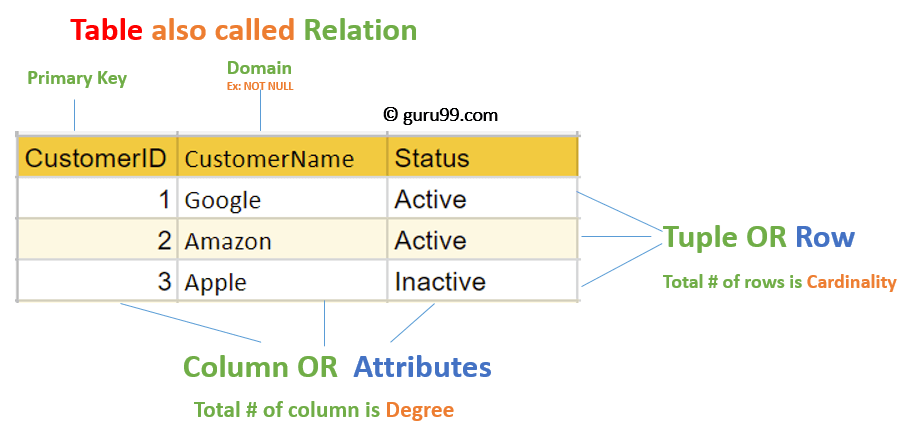
\includegraphics[width=\linewidth]{RelationalModel.jpg}
    \caption{Relational Model}
\end{figure}

\begin{description}
    \item[Attribute] Column
    \item[Relation] Table
    \item[Tuple] Row
    \item[Degree] Count(Column)
    \item[Cardinality] Count(Row)
    \item[Domain] 数据类型,约束等
    \item[Relation Key] 主键外键
    \item[Relation Schema] 表名 和 其中的列
    \item[Relation Instance] 表中的数据
\end{description}


\subsection{SQL}

Data Definition Language 定义

\begin{itemize}
    \item CREATE
    \item ALTER
    \item DROP
    \item TRUNCATE
\end{itemize}

Data Manipulation Language 操作

\begin{itemize}
    \item INSERT
    \item UPDATE
    \item DELETE
\end{itemize}

Data Control Language 权限

\begin{itemize}
    \item GRANT
    \item REVOKE
\end{itemize}

Transaction Control Language 事务

\begin{itemize}
    \item COMMIT
    \item ROLLBACK
    \item SAVEPOINT
\end{itemize}

Data Query Language 查询

\begin{itemize}
    \item SELECT
\end{itemize}


\subsection{索引}

Clustered Index

\begin{itemize}
    \item 行的物理与逻辑顺序相同
    \item 一个表只有一个
    \item Primary Key 默认
\end{itemize}

Non-clustered Index

\begin{itemize}
    \item 储存的是指向行的指针
    \item UNIQUE 默认
\end{itemize}

Covering Indexes

\begin{itemize}
    \item 索引中包含了要查询的字段
\end{itemize}


\subsection{Normalization}

消除冗余,inconsistent 的依赖关系


\subsubsection{不一致}

用户在 Customer 表中查找 Address 是合理的  
但是在这里查找 负责这个客户的 员工的 Salary 就不合理了  
这应该去 Employee 表中查找

不一致的依赖关系 会使数据难以访问

\begin{table}[H]
    \centering
    \begin{tabular}{|c|c|c|c|c|c|}
        \hline
        学号 & 教师 & 咨询室 & 课程 1 & 课程 2 & 课程 3 \\
        \hline
        S1 & T1 & R1 & C1 & C2 & C3 \\
        \hline
        S2 & T2 & R2 & C1 & C2 & C4 \\
        \hline
    \end{tabular}
\end{table}


\subsubsection{1NF}

每一个字段都是最小的,不包含其他字段,不重复

\begin{itemize}
    \item 消除重复的列
    \item 为相关数据单独建表
    \item 使用主键标识每组相关数据
\end{itemize}

\begin{table}[H]
    \centering
    \begin{tabular}{|c|c|c|c|}
        \hline
        学号 & 教师 & 咨询室 & 课程 \\
        \hline
        S1 & T1 & R1 & C1 \\
        \hline
        S1 & T1 & R1 & C2 \\
        \hline
        S1 & T1 & R1 & C3 \\
        \hline
        S2 & T2 & R2 & C1 \\
        \hline
        S2 & T2 & R2 & C2 \\
        \hline
        S2 & T2 & R2 & C4 \\
        \hline
    \end{tabular}
\end{table}


\subsubsection{2NF}

消除重复的行

\begin{itemize}
    \item 为应用于多条记录的值,创建单独的表
    \item 用外键连接这些表
\end{itemize}

Student

\begin{table}[H]
    \centering
    \begin{tabular}{|c|c|c|}
        \hline
        学号 & 教师 & 咨询室 \\
        \hline
        S1 & T1 & R1 \\
        \hline
        S2 & T2 & R2 \\
        \hline
    \end{tabular}
\end{table}

Course

\begin{table}[H]
    \centering
    \begin{tabular}{|c|c|}
        \hline
        学号 & 课程 \\
        \hline
        S1 & C1 \\
        \hline
        S1 & C2 \\
        \hline
        S1 & C3 \\
        \hline
        S2 & C1 \\
        \hline
        S2 & C2 \\
        \hline
        S2 & C4 \\
        \hline
    \end{tabular}
\end{table}


\subsubsection{3NF}

消除与主键无关的数据:咨询室是与学生编号无关的数据

Student

\begin{table}[H]
    \centering
    \begin{tabular}{|c|c|}
        \hline
        学号 & 教师 \\
        \hline
        S1 & T1 \\
        S2 & T2 \\
        \hline
    \end{tabular}
\end{table}

Teacher

\begin{table}[H]
    \centering
    \begin{tabular}{|c|c|}
        \hline
        教师 & 咨询室 \\
        \hline
        T1 & R1 \\
        T2 & R2 \\
        \hline
    \end{tabular}
\end{table}


\subsubsection{Boyce-Codd}

在 3NF 的基础上,每个属性都不传递依赖

StorehouseManage (WarehouseID, ItemID, AdminID, Num)

每个管理员只在一个仓库工作,一个仓库储存多个物品,则存在关系

\begin{itemize}
    \item (WarehouseID, ItemID) $\to$ (AdminID, Num)

    \item (AdminID, ItemID) $\to$ (WarehouseID, Num)
\end{itemize}

所以有两组候选关键字,唯一非关键字是 Num,符合 3NF,但是存在 (WarehouseID) $\leftrightarrow$ (AdminID) 关键字决定关键字的情况,循环传递依赖

异常:

\begin{description}
    \item[删除] 清空仓库会导致 WarehouseID AdminID 被删除

    \item[插入] 仓库无物品时,无法分配管理员

    \item[更新] 换管理员,则修改全表
\end{description}

修改:

\begin{itemize}
    \item StoreManage (WarehouseID, AdminID)

    \item Warehouse (WarehouseID, ItemID, Num)
\end{itemize}


\subsubsection{4NF}

消除 Multi-Valued Dependency,最简单的是多对多


\subsection{Entity Relationship}

\begin{description}
    \item[Entity] 矩形,表
    \item[Attribute] 椭圆,列
    \item[Relationship] 菱形,表之间的关系
    \item[Computed] 虚线,计算得出的属性
    \item[Multi Value] 双椭圆,多值属性
    \item[Optional] 可选属性
    \item[Composite] 矩形内加一个菱形,多对多联系
    \item[Weak] 双层矩形,依赖另一个实体存在
\end{description}

\begin{figure}[H]
    \centering
    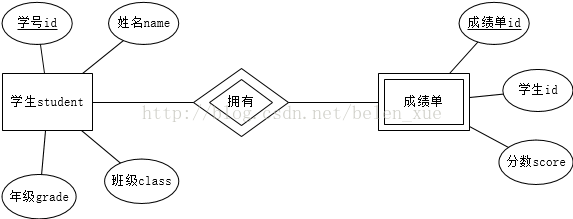
\includegraphics[width=\linewidth]{ER2.png}
\end{figure}

\begin{figure}[H]
    \centering
    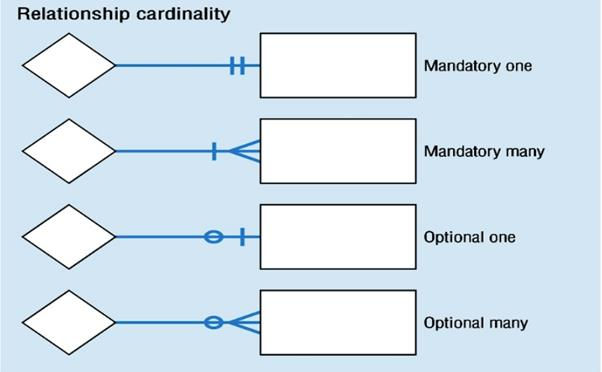
\includegraphics[width=\linewidth]{ER.jpg}
\end{figure}

画图步骤

\begin{enumerate}
    \item Entity Identification 找实体
    \item Relationship Identification 找关系
    \item Cardinality Identification 一对多之类的
    \item Identify Attributes 找列
    \item Create ER Diagram 画图
\end{enumerate}


\subsection{数据仓库}

Online Analytical Processing,使用数据库系统来帮助洞察业务,如 Redshift,主要用于数据分析

数据仓库是为只读优化的

\begin{description}
    \item[事实表] 含有大量的数据,并且是可以汇总,并被记录的

    \item[维度表] 分析数据的窗口,包含事实表中记录的属性

    \item[Star] 一张事实表和多张维度表组成

    \item[Snowflake] 每一个维度表都可以向外连接多个子维度表

    \item[Galaxy] 多个事实表版本的星型模型,多张事实表共用模型中的维度表
\end{description}


\subsubsection{Data Cube}

表示那些很大的数据集合,储存多维度数据

\begin{figure}[H]
    \centering
    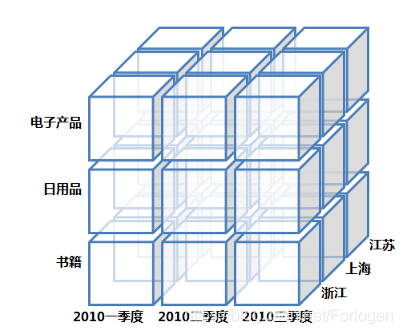
\includegraphics[width=\linewidth]{Cube.png}
\end{figure}

\begin{description}
    \item[Drill Down] 季度总销售 $\to$ 每个月

    \item[Roll Up] 4 5 6 月 $\to$ 第二季度

    \item[Slice] 只分析电子产品

    \item[Dice] 第一和第二季度

    \item[Rotate] 产品与地区互换维度
\end{description}

\begin{figure}
    \centering
    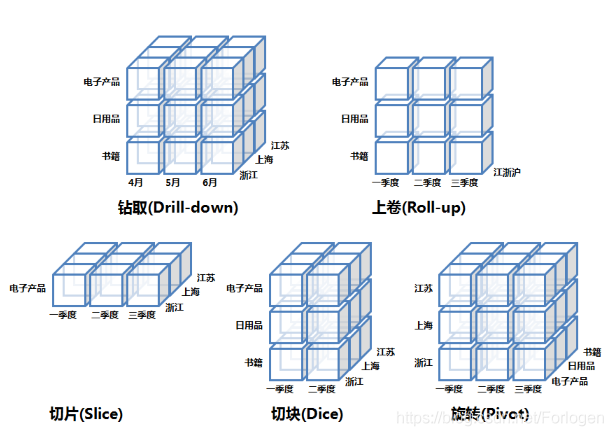
\includegraphics[width=\linewidth]{Action.png}
\end{figure}


\section{Algorithms \& Data Structures}


\subsection{The concept of algorithms, the description of an algorithm}

算法类似于食谱,每一步都是为了达成预期而需要采取的具体行动,其包括一组输入,并对输入进行操作,产生输出。它必须定义明确,有具体目的,且能在合理时间使用合理资源完成任务。


\subsection{Turing machines}

\url{https://Aloen.to/Algorithm/TM/Turing-Machines/}

\begin{itemize}
    \item abstract models for real computers having an infinite memory (in the form of a tape) and a reading head

    \item has finite number of internal states

    \item has distinguished starting and final states

    \item has transition functions
\end{itemize}

\begin{itemize}
    \item accepts the initial content of the tape if it terminates in an accepting state

    \item 如果没有匹配的规则,则终止

    \item 如果对某个状态和输入符号集,有多个匹配规则,则 Non-Deterministic

    \item 所有的 ND 都有等价的 确定
\end{itemize}


\subsubsection{Halting Problem}

属于 Computability Theory,判断任意一个程序是否能在有限的时间之内结束运行。Traveling Salesman Problem 不是


\subsection{Efficiency of algorithms, basics of complexity theory}

算法会消耗时间和内存,复杂度就是衡量消耗的指标


\subsubsection{时间复杂度}

时间复杂度主要是循环导致的,O 表示了增长变化趋势,下面列出的复杂度递增,效率递减

\begin{description}
    \item[常数阶 $O(1)$] ~

    \begin{minted}{js}
        let i = 1;
        i = i + 1;
    \end{minted}

    没有循环

    \item[对数阶 $O(\log N)$] ~

    \begin{minted}{js}
        let i = 1;
        while (i < n)
          i = i * 2;
    \end{minted}

    循环 x 次后,i > n,则 $2^x > n$,即 $x > \log_2 (n)$

    \item[线性阶 $O(N)$] ~

    \begin{minted}{js}
        for (let i = 0; i < n; i++)
          console.log(i);
    \end{minted}

    循环 n 次

    \item[线性对数阶 $O(N \log N)$] ~

    \begin{minted}{js}
        for (let i = 1; i < n; i = i * 2)
          for (let j = 0; j < n; j++)
            console.log(j);
    \end{minted}

    把 $O(\log N)$ 的代码,再循环 N 次

    也可以把 $O(N)$ 的代码,再循环 $\log N$ 次

    \item[平方阶 $O(N^2)$] ~

    \begin{minted}{js}
        for (let i = 0; i < m; i++)
          for (let j = 0; j < n; j++)
            console.log(j);
    \end{minted}

    把 $O(N)$ 的代码,再循环 N 次

    当然也可以是 $m \times n$
\end{description}

其他的包括但不限于

\begin{itemize}
    \item K 次方阶 $O(N^k)$

    \item 指数阶 $O(2^N)$ 一般是递归算法

    \item $O(3^N)$
\end{itemize}


\paragraph{计算} ~

$T(n)$:算法的执行次数

$T(n) = O(f(n))$

\begin{description}
    \item[嵌套循环] ~

    由内向外分析,并相乘

    \begin{minted}{js}
        // O(n)
        for (let i = 0; i < n; i++)
          // O(n)
          for (let j = 0; j < n; j++)
            console.log(j); // O(1)
    \end{minted}

    时间复杂度为 $O(n \times n \times 1) = O(n^2)$

    \item[顺序执行] ~

    把它们的时间复杂度相加
    
    不要求精度 = 最大的时间复杂度

    \begin{minted}{js}
        // O(n)
        for (let i = 0; i < n; i++)
          console.log(i);

        // O(n^2)
        for (let i = 0; i < n; i++)
          for (let j = 0; j < n; j++)
            console.log(j);
    \end{minted}

     $O(n + n^2)$ 或 $O(n^2)$

    \item[条件分支] ~

    最麻烦的那个情况

    \begin{minted}{js}
        if (n > 10)
          // O(n)
          for (let i = 0; i < n; i++)
            console.log(i);
        else
          // O(1)
          console.log(n);
    \end{minted}

    $O(n)$
\end{description}


\subsubsection{空间复杂度}

\begin{description}
    \item[$O(1)$] ~

    \begin{minted}{js}
        let i = 1;
        i = i + 1;
    \end{minted}

    变量所分配的空间,都不随数据量的变化而变化

    \item[$O(N)$] ~

    \begin{minted}{js}
        let arr = [];
        for (let i = 0; i < n; i++)
          arr.push(i);
    \end{minted}

    看到数组就表明,空间是随着 n 增大而增大的
\end{description}

所以,如果 n 增大,程序占用的空间

\begin{itemize}
    \item 不变,$O(1)$

    \item 成线性增长,$O(N)$

    \item 成平方增长,$O(N^2)$
\end{itemize}

以此类推,也有 $O(N + M)$, $O(\log N)$等


\subsection{Approaches to algorithm construction}

\begin{description}
    \item[Brute Force] 尝试所有可能方案,直到可行,不一定有效

    \item[Divide and Conquer] 将问题分解成多个子问题,并分别解决,再结合起来

    \item[Greedy] 对每一步做出 Locally Optimal 解,但不一定是全局最优

    \item[Dynamic Programming] 动态规划,试图仅解决每个子问题一次,从而减少计算量,对有重复子问题非常有效

    \item[Backtracking] 寻找所有解决方案,依次尝试,当不正确时,进行回溯

    \item[Randomized] 如随机化寻找优化问题的近似解
\end{description}


\subsection{Linear data structures}

\begin{description}
    \item[Lists] 一种特定类型的集合,有序可重复,用数组或链表

    \item[Collections] 任何元素的分组,可能有序 / 无序,重复 / 唯一,各种数据结构 Set Map
    
    \item[First-In-First-Out] Queue,先进先出
    
    \item[Last-In-First-Out] Stack,后进先出
    
    \item[Binary Heap] 是完全二叉树,从左到右填充
\end{description}

\url{https://Aloen.to/Algorithm/Basics-of-Computer-Science/#Sorting-algorithms-and-their-complexity}


\subsection{Search in hash tables}

储存键值对,O(1),先将数据映射成它的哈希值

解决碰撞:

\begin{description}
    \item[Separate Chaining] 将哈希值相同的数据元素存放在一个链表中,当查找到这个链表时,必须采用线性查找,需要额外空间和时间

    \item[Open Addressing] 如果两个数据元素的哈希值相同,会生成另一个哈希值,容易出现哈希值被连续占用,不适用于大量数据
\end{description}


\subsection{Binary Search Tree}

在二叉查找树中:

\begin{itemize}
    \item 左子树所有节点小于根节点

    \item 右子树所有节点大于根节点

    \item 任意子节点均为二叉查找树

    \item 没有相同的节点
\end{itemize}

\begin{figure}[H]
    \centering
    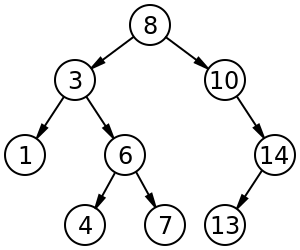
\includegraphics[width=0.5 \linewidth]{BST.png}
\end{figure}

在树种查找只需要判断节点大小。左下最小,右下最大


\subsubsection{删除节点}

删除一个节点,还要让 BST 保持正确结构

\begin{itemize}
    \item 没有子树,直接删掉

    \item 只有单侧子树,孩子顶替

    \item 左右子树,后继节点顶替
\end{itemize}

后继节点就是在中序遍历时的下一个节点。找 A 的后继节点,则从 A 的右子树开始,一路向左走,走到没有左子树为止


\subsection{234 / RB Tree}

BV1BB4y1X7u3 / BV1Ce4y1Q76H


\section{Graph Algorithms}


\subsection{The concept of a graph, its representations and visualization}

$G=(V,E)$ where V is finite and not empty set, V = edges, E = vertices

Graph Representations

\begin{itemize}
    \item Drawing
    \item Edge and Vertex List
    \item Adjacency Matrix
\end{itemize}

\begin{figure}
    \centering
    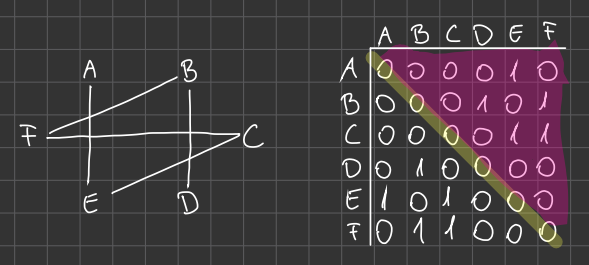
\includegraphics[width=\linewidth]{1.png}
\end{figure}


\subsection{Euler Path}

欧拉路径也就是一笔画问题,回路则需要回到起点

它遍历每条边,顶点可以经过多次

对于无向图:

\begin{description}
    \item[Path] 奇数度数的点只能有 0 个或 2 个

    \item[Circuit] 不能有奇数度数点
\end{description}

对于 Directed:

\begin{description}
    \item[Path] 出等于入 or 起点出比入多 1,终点入比出多 1,其余的相等

    \item[Circuit] 出等于入
\end{description}


\subsubsection{Hierholzer}

算法,$O(V + E)$

\begin{enumerate}
    \item 从有欧拉路径的点出发

    \item 深度优先遍历整个图,经过的顶点不再遍历

    \item 若点没有可遍历的邻居,将此点入栈,并删除
\end{enumerate}


\subsection{Hamiltonian Path}

哈密顿路径强调的是经过每个顶点一次,是 NP 完全问题,一般使用枚举

回溯搜索是深度优先搜索的一种,但在求解过程中不保留完整的树结构,而 DFS 则记下完整的搜索树

对于求路径来说,起始点是谁很重要,同一个图,从有的起始点出发就存在,从有的起始点出发就不存在


\subsection{Tree Graphs}

树是一种无向、无循环的连接图,在树的任何两个顶点之间都有唯一的路径


\subsection{Fundamental graph algorithms}

\begin{description}
    \item[Pre] XLR
    \item[Mid] LXR
    \item[Post] LRX
\end{description} 

\begin{figure}
    \centering
    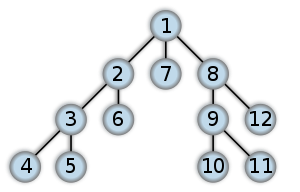
\includegraphics[width=\linewidth]{DFS.png}
    \caption{Depth-First-Search}
\end{figure}

\begin{figure}
    \centering
    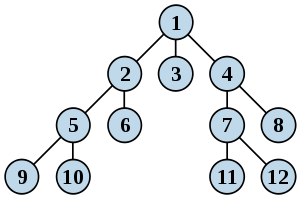
\includegraphics[width=\linewidth]{BFS.png}
    \caption{Breadth-First Search}
\end{figure}


\subsection{Optimal spanning trees}

最小生成树问题是指在一个加权无向连通图中找到一棵包含所有节点且边的权值和最小的生成树


\subsubsection{Prim}

贪心算法 $O(V^2)$

\begin{enumerate}
    \item 选择一个顶点作为起点

    \item 选择所有与生成树相邻中权重最小的一条边
\end{enumerate}

\url{https://zh.wikipedia.org/wiki/普林姆算法#例示}


\subsubsection{Kruskal}

贪心算法 $O(E \log V)$

\begin{enumerate}
    \item 将所有边从小到大排序

    \item 依次选择边,如果该边的两个顶点不在同一个连通块中,则加入
\end{enumerate}

\url{https://zh.wikipedia.org/wiki/克鲁斯克尔演算法#示例}


\subsection{Shortest paths}

最短路径算法是用来寻找带有加权边的图中两个顶点之间的最短路径


\subsubsection{Dijkstra}

\begin{minted}{js}
A --5-- B
|       |
4       6
|       |
C --5-- D
\end{minted}

首先,将 A 设为原点,并初始化每个顶点到原点的距离为 \infty

\begin{minted}{js}
/** 每个顶点到原点的距离 */
let dist: Record<string, number> = {
  A: 0,
  B: Infinity,
  C: Infinity,
  D: Infinity,
};

/** 获取两个顶点之间的权重 */
declare function weight(node1: string, node2: string): number;
\end{minted}

接下来,不断迭代更新每个点到原点的最短距离。在每次迭代中,首先找到所有未被更新的点中距离原点最近的点,然后更新它到原点的最短距离,并根据新的距离,更新其他点到原点的距离

从 A 向外扩散

\begin{minted}{js}
dist.B =
  Math.min(dist.B, dist.A + weight("A", "B")) =
  Math.min(Infinity, 0 + 5) =
    5;

dist.C =
  Math.min(dist.C, dist.A + weight("A", "C")) =
  Math.min(Infinity, 0 + 4) =
    4;
\end{minted}

从 B 向外扩散

\begin{minted}{js}
dist.D =
  Math.min(dist.D, dist.B + weight("B", "D")) =
  Math.min(Infinity, 5 + 6) =
    11;
\end{minted}

从 C 向外扩散

\begin{minted}{js}
dist.D = 
  Math.min(dist.D, dist.C + weight("C", "D")) = 
  Math.min(11, 4 + 5) = 
    9;
\end{minted}

得到结果

\begin{minted}{js}
dist = {
  A: 0,
  B: 5,
  C: 4,
  D: 9,
};
\end{minted}

所以,从 A 到 D 的最短距离为 9


\subsection{Bellman-Ford}

求含负权图的单源最短路径,遍历全图 V - 1 次,能缩小距离的就缩小

BV1j34y1s7d8


\section{Programming}


\subsection{Arithmetical and logical operations}

\begin{description}
    \item[算数] \verb|+ - * / % ++ --|

    \item[关系] \verb|== != > < >= <=|

    \item[逻辑] \verb|&&| || !

    \item[位] \& | ~ \verb|^ << >>|

    \item[赋值] \verb|= += -= *= /=|
\end{description}


\subsection{Control structures (conditional and unconditional flow control, loops)}

\begin{description}
    \item[条件语句] if else switch

    \item[循环] for in of do while break continue
\end{description}


\subsection{Functions and procedures (subprograms, subroutines)}

Function:Subprograms,重用代码块,执行特定任务

Procedure:Subroutine,不返回一个值,通过副作用


\subsection{data passing}

\begin{description}
    \item[按值传递] 传递副本
    \item[按引用传递] 传递指针
    \item[ref] 按引用传递值类型 
    \item[int[]] 按值传递引用类型 
\end{description}


\subsection{local and global variables}

\begin{description}
    \item[local] 在作用域内声明,会销毁

    \item[global] 可以从任何部分访问
\end{description}


\subsection{the role of stacks in function calls}

Call Stack 是管理函数调用关系的结构,保证调用顺序和追踪


\subsubsection{Stack Frame}

函数的参数和局部变量等储存在 Stack Frame 中,并入 Call Stack,当执行完毕后弹出,包含了函数的执行环境,包括:Function Parameters、Local Variables、Return Address


\subsubsection{Function Call}

当函数被调用时

\begin{enumerate}
    \item 返回地址(函数结束后的指令)入栈
    \item 参数入栈
    \item 跳转到函数起始位置,进入函数
    \item 创建新的 Stack Frame,局部变量 Allocated
    \item 执行
\end{enumerate}


\subsubsection{Function Return}

当函数执行完毕,准备返回时

\begin{enumerate}
    \item 如果函数有返回值,它被储存在特定位置,供调用者访问
    \item 函数的 Frame 从调用栈弹出,局部变量和参数被销毁
    \item 跳到返回地址,继续执行
\end{enumerate}


\subsubsection{Recursion}

当函数直接或间接调用自己,每一次调用都会创建新的 Stack Frame。调用栈的大小是有限制的。当递归层数过深或者函数调用过多时,调用栈可能会溢出


\subsection{Basics of object-oriented programming: classes, objects, inheritance, polymorphism, encapsulation}

\begin{description}
    \item[Objects] 是类的实例化结果

    \item[多态] Polymorphism 一个对象表现出多种形态 \\ virtual abstract interface 可重用性和灵活性

    \item[封装] Encapsulation 将数据和相关的行为封装在类中,并对外部隐藏实现细节 访问修饰符
\end{description}


\section{Compilers}


\subsection{Chomsky Classification}

\begin{table}[h]
\centering
\begin{tabular}{|c|c|c|c|}
\hline
文法 & 语言 & 类型 & 产生式规则 \\
\hline
0 & 递归可枚举 & 图灵机 & $\alpha \rightarrow \beta$ \\
\hline
1 & 上下文相关 & 线性有界非确定图灵 & $\alpha A \beta \rightarrow \alpha \gamma \beta$ \\
\hline
2 & 上下文无关 & 非确定下推自动机 & $A \rightarrow \gamma$ \\
\hline
3 & 正则 & 有限状态自动机 & $A \rightarrow aB$ \\
& & & $A \rightarrow a$ \\
\hline
\end{tabular}
\end{table}


\subsection{Regular Languages}

\begin{itemize}
    \item 空集合 Ø 是正则语言
    \item 只包含一个空串 $\epsilon$ 的是正则语言
\end{itemize}


\subsection{relation to lexical analyzer programs}

Tokenizer 将一连串的符号分解为一连串的标记,然后传递给 Parser,生成 AST

正则语言可以描述定义编程语言符号的模式和规则,正则表达式是一种方式

\url{https://juejin.cn/post/6844904035271573511}


\subsection{Finite automata}

Finite-State Machine 被用来识别正则语言

\begin{description}
    \item[Deterministic] 对每个状态和输入都有确定的下一个状态

    \item[Nondeterministic] 可以到不同的下一个状态,有 $\epsilon$ 过度,不消耗输入
\end{description}


\subsection{The structure of compilers}

翻译高级代码至低级语言

\begin{description}
    \item[Lexical] 词法分析
    \item[Syntax] 语法分析,AST
    \item[Semantic] 检查语法正确,类型检查等
    \item[Intermediate] 与平台无关的中间代码
    \item[Optimization] 提高性能等
    \item[Generation] 生成目标机器码
\end{description}


\subsection{the process of compilation or interpretation}

\begin{description}
    \item[Compilation] 代码在执行前被翻译成机器码,运行的快

    \item[Interpretation] 解释,直接执行源码,JS
\end{description}

Java 之类使用 IL,预编译


\subsection{Look-Ahead}

在 parsing 阶段,根据 parser 的当前状态来预测输入,在出现歧义的情况下应用哪条规则,理解更复杂的语法,k 代表可以提前看的标记数量

\begin{description}
    \item[LL(k)] top-down,Left-to-right, Leftmost derivation

    \item[LR(k)] bottom-up,L2R, Rightmost derivation
\end{description}


\section{System Engineering}


\subsection{Basics of UML}

Unified Modeling Language,用图形符号描述系统结构,行为,相互作用

\begin{description}
    \item[Class] 属性,方法,关系,约束,静态结构
    
    \item[Object] 快照,类的实例

    \item[Use Case] Actors 和 功能的交互

    \item[Sequence] 按照时间说明对象间的互动

    \item[Component] 模块,库之类的依赖关系
\end{description}


\subsection{Meta-models}

The underlying framework or language used to define and describe the construct and rules of UML. 它定义了 UML 的 syntax and semantics,用于解释模型


\subsection{The 4-layer meta-model of UML}

\begin{description}
    \item[M0] Run-Time instances,代表实际运行中存在的具体对象和数据

    \item[M1] User model,用户对系统的理解,如何互动,期望,目标和任务

    \item[M2] UML 抽象,用来定义 meta models

    \item[M3] Meta-Object Facility,最高抽象
\end{description}


\subsection{Basics of workflow modeling}

\begin{description}
    \item[Identify Boundaries] 要建模的内容,范围,输入输出等

    \item[Define Objectives] 确定模型目标,期望的结果,限制等

    \item[Identify Components] 确定组成部分

    \item[Establish Relationships] 确定关系和依赖

    \item[Model Structure] 使用图形符号来表示

    \item[Specify Logic] 确定条件判断,循环,异常处理等

    \item[Iterate and Refine] 继续完善
\end{description}


\subsection{The Software Process Engineering Model (SPEM) UML profile describes the classic and RUP methodologies steps}


\subsubsection{Classic Waterfall}

\begin{description}
    \item[Requirements Analysis] 

    \item[System Design] 

    \item[Implementation] 

    \item[Testing and Integration] 

    \item[Deployment] 

    \item[Operation and Maintenance] 
\end{description}


\subsubsection{Rational Unified Process}

\begin{description}
    \item[Inception] 确定范围,目标,风险,提案,可行性

    \item[Elaboration] 确定优先次序,设计系统结构,企划案

    \item[Construction] 实现系统,测试,审查

    \item[Transition] 验收测试,部署
\end{description}


\subsection{Programming and software engineering technologies and methodologies}

\begin{description}
    \item[Programming Languages] Java
    
    \item[Integrated Development Environments] VS IDEA

    \item[Version Control Systems] GIT

    \item[Agile Methodologies] Kanban

    \item[DevOps] Continuous Integration / Delivery

    \item[Software Development Lifecycle] Waterfall
\end{description}


\subsection{Procedural techniques}

编程范式,OOP 是一种

\begin{description}
    \item[Modular Programming] ~

    \begin{itemize}
        \item Modularization
        \item Encapsulation
    \end{itemize}

    \item[Control Structures] ~

    \begin{itemize}
        \item Sequence
        \item Selection
        \item Iteration
    \end{itemize}

    \item[Abstraction] 

    \item[Variable Scope and Lifetime] 

    \item[Error Handling] 
\end{description}


\end{document}
